\documentclass[conference]{IEEEtran}

%%% PACKAGES %%%
% Typesetting
\usepackage[T1]{fontenc}
\usepackage[utf8]{inputenc}
\usepackage[english]{babel}
%\usepackage{lmodern} % latin modern font
\usepackage{csquotes} % pro­vides ad­vanced fa­cil­i­ties for in­line and dis­play quo­ta­tions (better to load when using biblatex)
\usepackage{textcomp} % pro­vide many text sym­bols (such as baht, bul­let, copy­right, mu­si­cal­note, onequar­ter, sec­tion, and yen), in the TS1 en­cod­ing
%\usepackage{setspace}
%\onehalfspacing % 1.5 linespaceing
%\usepackage{fancyhdr} % pro­vides ex­ten­sive fa­cil­i­ties, both for con­struct­ing head­ers and foot­ers, and for con­trol­ling the

\usepackage{siunitx}
\sisetup{
	group-digits = integer, % only group digits (by three) for integers (not decimals)
	binary-units = true, % load binary units
	detect-all
}
%\usepackage{enumitem}
%\setlist[enumerate]{label*=\arabic*.,topsep=0pt,partopsep=0pt,parsep=0pt,itemsep=0pt}
%\setlist[itemize]{topsep=0pt,partopsep=0pt,parsep=0pt,itemsep=0pt}
%\usepackage{bigfoot} % The pack­age aims to pro­vide a ‘one-stop’ so­lu­tion to re­quire­ments for foot­notes
%\usepackage{afterpage} % to use \footnotemark and \footnotetext in captions for special cases
\usepackage{algorithm} % the al­go­rithm pack­age de­fines a float­ing al­go­rithm en­vi­ron­ment de­signed to work with the al­go­rith­mic style
\usepackage{algorithmic}
%\usepackage{algpseudocode} % The algorithmicx package provides many possibilities to customize the layout of algorithms.
\usepackage{newunicodechar}
\usepackage{pifont}

% Math
\usepackage{amsmath}
\usepackage{amsfonts}
\usepackage{amssymb}
\usepackage{amsthm}
\usepackage{bm}
%\usepackage{mathtools}

% Figures
\usepackage{graphicx}
\graphicspath{{figures/}}
\usepackage{xcolor}
%\usepackage[font=small, labelfont=bf, format=plain, labelsep=space, figurename=Figure, tablename=Table, skip=5pt]{caption}
%\usepackage[labelfont=rm, labelformat=parens, labelsep=space, skip=2pt]{subcaption}
\usepackage[skip=2pt]{subcaption}
%	IEEE caption set-up
\captionsetup[figure]{name=Fig.}
\captionsetup[table]{name=TABLE, font=footnotesize, labelfont=up, textfont=sc, labelsep=newline, justification=centering}
\captionsetup[subfigure]{labelformat=simple}
\renewcommand*{\thesubfigure}{(\alph{subfigure})} % adds parens around subfigure label for clean subreference using \ref{} or \subref{}. Must be used with subcaption options, labelformat=simple and subrefformat=simple (not sure to be required...)
\usepackage{tikz}
%\usepackage{pgfgantt}

% Tables
\usepackage{multirow}
%\usepackage{adjustbox}
%\usepackage{makecell}
\usepackage{longtable} % use of \linebreak instead of \\ in headers to avoid a bug with longtables (or longtabu) across two pages
\usepackage{tabu}
%	\tabulinesep = 4pt
	\tabcolsep = 4pt
\usepackage{booktabs}
%\usepackage{colortbl}

% Others
%\usepackage[draft]{pdfpages} % include pdf pages
\usepackage{calc}
%\usepackage{rotating}
\usepackage{todonotes} % \todo, \missingfigures and \listoftodos
\usepackage{xifthen} % This pack­age ex­tends the ifthen pack­age by im­ple­ment­ing new com­mands to go within the first ar­gu­ment of \ifthenelse
\usepackage{xparse} % The pack­age pro­vides a high-level in­ter­face for pro­duc­ing doc­u­ment-level com­mands. 
\usepackage{etoolbox} % The package is a toolbox of programming facilities geared primarily towards LaTeX class and package authors. 
\usepackage{xstring}
\usepackage{xspace} % useful for newcommands and spacing

% References and URLs
\usepackage{cleveref}
\crefname{table}{Table}{Tables} % default: table
\crefname{figure}{Fig.}{Fig.} % default: figure
\crefname{section}{Section}{Section} % default: section
\crefname{equation}{Equation}{Equation} % default: eq.
\usepackage{url}


%%% TIKZ %%%
% *** TIKZ PACKAGES ***
\usepackage{xparse}
\usepackage{tikz}
\usetikzlibrary{shapes, arrows.meta, decorations.pathmorphing}
\usetikzlibrary{calc, positioning}
\usetikzlibrary{backgrounds}
\usetikzlibrary{intersections} % provides name path=
\usetikzlibrary{angles} % provides pic angle

\usepackage{etoolbox}

% Tikzset
\tikzset{%
	block/.style = {draw, shape=rectangle, thick, minimum height=2em, minimum width=2em},
	sum/.style = {draw, shape=circle, thick, inner sep=0pt},
	conn/.style={fill, shape=circle, minimum size=0.1cm, inner sep=0, outer sep=0},
	inout/.style={inner sep=0, outer sep=0},
	dot/.style={fill=, shape=circle, minimum size=\pgflinewidth, inner sep=0, outer sep=0},
	param/.style={inner sep=0, outer sep=1pt},
	loosely dotted round/.style={dash pattern=on 0pt off 6\pgflinewidth, line cap=round},
	%	transducer/.style = {shape=rectangle, draw=black, fill=black!20!white, thick, minimum height=0.15cm, minimum width=0.30cm, inner sep=0pt},
	%	my funny rectangle/.style n args={4}{%
	%    rectangle,
	%    draw,
	%    fit={(#1,#3) (#2,#4)}
	%%    append after command={\pgfextra{\let\mainnode=\tikzlastnode}
	%%      node[above right] at (\mainnode.north west) {#3}%
	%%      node[above left] at (\mainnode.north east) {#4}%
	%%      node[below left] at (\mainnode.north west) {#1}%
	%%      node[above left] at (\mainnode.south west) {#2}%
	%%    },
	%  }
}

%\def\td_number{3}

%\newcommand*{\transducer}[4][-1][-2]{\path[draw=black, fill=black!20!white] (#3, #1) rectangle (#4, #2)}

% arg1: lx (optional, default=1)
% arg2: ly (optional, default=2)
% arg3: x_center
% arg4: y_center
%\NewDocumentCommand{\transducer}{ O{-1} O{-2} m }{\path[draw=black, fill=black!20!white] (#3, #1) rectangle (#4, #2)}

\NewDocumentCommand{\rectangle}{ m m }{%
	%\newlength{\Xone}{#1 cm}%\pgfmathparse{#1+1}\pgfmathresult
	\path[draw=black, fill=black!20!white] #1 rectangle #2
}

%\pgfdeclarelayer{bg}    % declare background layer
%\pgfsetlayers{bg,main}  % set the order of the layers (main is the standard layer)

% This bascially automates a \newcommand{<name>}{} to ensure
% that a command with the given <name> does not already exist
\newcommand*{\pgfmathsetnewmacro}[2]{%
	\newcommand*{#1}{}% Error if already defined
	\pgfmathsetmacro{#1}{#2}%
}%

% Transducer commands
\newcommand*{\transducerNumb}{10}
\newcommand*{\transducerWidth}{0.75}
\newcommand*{\transducerHeight}{0.25}
\newcommand*{\transducerInitXPos}{3}
\newcommand*{\transducerXOffset}{1}
\definecolor{transducer-color}{gray}{0.8}
\newcommand*{\transducerLabeled}{9}
\newcommand*{\transducerLabeledBis}{7}

% Measurement commands
\newcommand*{\measurementLength}{6}
\definecolor{measurement-color}{gray}{0.7}

% Insonified domain
\pgfmathsetmacro{\domainXMin}{\transducerInitXPos}
\pgfmathsetmacro{\domainXMax}{12}
\pgfmathsetmacro{\domainZMin}{1}
\pgfmathsetmacro{\domainZLength}{7}
\pgfmathsetmacro{\domainZMax}{\domainZMin+\domainZLength}
\pgfmathsetmacro{\domainDxOffset}{1}
\pgfmathsetmacro{\domainDzOffset}{1}
\definecolor{domain-color}{gray}{0.7}
\definecolor{scatterer-color}{gray}{0}

% Wavefront and time of flight
\definecolor{wavefront-color}{gray}{0.5}

% Axes
\newcommand*{\axesOffset}{1.5}

% Conics
\definecolor{conic-color}{gray}{0}
% 	Ellipse
% http://tex.stackexchange.com/questions/75017/draw-an-ellipse-from-the-two-focus-points-foci-and-the-sum-of-the-distances-fr
\newcommand*{\ellipsebyfoci}[4]{% options (draw, fill, color, etc.), focus pt1, focus pt2, cste
	\path[#1] let \p1=(#2), \p2=(#3), \p3=($(\p1)!.5!(\p2)$)
	in \pgfextra{
		\pgfmathsetmacro{\angle}{atan2(\x2-\x1,\y2-\y1)}
		\pgfmathsetmacro{\distfoci}{veclen(\x2-\x1,\y2-\y1)/1cm} % convert back to cm
		\pgfmathsetmacro{\axeone}{#4/2}
		\pgfmathsetmacro{\axetwo}{sqrt(\axeone^2 - (0.5*\distfoci)^2)}
%		\pgfmathsetmacro{\focal}{veclen(\x2-\x1,\y2-\y1)/2/1cm}
%		\pgfmathsetmacro{\lentotcm}{\focal*2*#4}
%		\pgfmathsetmacro{\axeone}{(\lentotcm - 2 * \focal)/2+\focal}
%		\pgfmathsetmacro{\axetwo}{sqrt((\lentotcm/2)*(\lentotcm/2)-\focal*\focal}
	}
%	(\p3) ellipse[x radius=\axeone cm,y radius=\axetwo cm, rotate=\angle];
	(\p3) ellipse[x radius=\axeone,y radius=\axetwo, rotate={90-\angle}];
%	(\p1) -- node[midway, sloped, above]{\distfoci} (\p2);
}

%%% NEW COMMANDS %%%
% Typesetting
\newcommand{\keywords}[1]{\noindent\textbf{Keywords:} #1}

% Math
\newcommand*{\abs}[1][]{\left\lvert#1\right\rVert}
\newcommand*{\norm}[2][]{\left\lVert#2\right\rVert_{#1}}
\newcommand*{\zeronorm}[1]{\norm[0]{#1}}
\newcommand*{\onenorm}[1]{\norm[1]{#1}}
\newcommand*{\twonorm}[1]{\norm[2]{#1}}
\newcommand*{\twoonenorm}[1]{\norm[2,1]{#1}}
\newcommand*{\fronorm}[1]{\norm[F]{#1}}
\newcommand*{\infnorm}[1]{\norm[\infty]{#1}}
\newcommand*{\pnorm}[1]{\norm[p]{#1}}
\newcommand*{\tvnorm}[1]{\norm[TV]{#1}}

% Sets
\newcommand*{\C}{\mathbb{C}}
\newcommand*{\R}{\mathbb{R}}
\newcommand*{\Q}{\mathbb{Q}}
\newcommand*{\Z}{\mathbb{Z}}
\newcommand*{\N}{\mathbb{N}}

% argmin, argmax, ...
\DeclareMathOperator*{\argmin}{argmin} % the star-version allows to have limit typeset bellow
\DeclareMathOperator*{\argmax}{argmax} % the star-version allows to have limit typeset bellow
% Matrix, vector, transpose, adjoint, ...
\newcommand*{\mat}[1]{\mathsf{#1}}
\newcommand*{\adjmat}[1]{\mathsf{#1}^T}
\renewcommand*{\vec}[1]{\bm{#1}}
\newcommand*{\tran}{^\mathsf{T}}
%\newcommand*{\tran}{^\intercal}
%\newcommand*{\tran}{^{\scriptscriptstyle\top}}
%\newcommand*{\tran}{\mkern-1mu{}_{}^{\scriptscriptstyle\top}\mkern-4mu}
\newcommand*{\conj}{^*}
\newcommand*{\adj}{^\dagger}
% Function, functional, ...
\newcommand*{\fun}[1]{#1}
\newcommand*{\funal}[1]{\mathcal{#1}}
% Transform, Dictionary, ...
\newcommand*{\dict}{\mat{D}}
\newcommand*{\transf}{\mat{\Psi}}
% Such that, subject to,...
\newcommand*{\suchthat}{\mid}
\newcommand*{\subjectto}{\,\,\mathrm{s.t.}\,\,}
\newcommand{\ser}[2]{#1^#2}

% US specific
\newcommand*{\medium}{\Omega}
\newcommand*{\transducer}{\Pi}
\newcommand*{\reflectivity}{\gamma}
\newcommand*{\rawdata}{m}
\newcommand*{\eaimpulseresp}{\fun{h_{el-ac}}}
\newcommand*{\excitation}{\fun{e}}
\newcommand*{\htx}{\fun{h_{Tx}}}
\newcommand*{\hrx}{\fun{h_{Rx}}}
\newcommand*{\pewavelet}{\fun{v_{pe}}}
\newcommand*{\eldir}{o}
\newcommand*{\wavelength}{\lambda}
\newcommand*{\noise}{n}

% Citations and referencs
%\newcommand*{\myciteauthor}[1]{\citeauthor{#1}~\cite{#1}}

% Latin expressions
% 	.\@ -> abbretiation period (for correct spacing)
\newcommand{\etc}{etc.\xspace}
\newcommand{\ie}{i.e.\@\xspace} % i.e. should NOT be italicized
\newcommand{\eg}{e.g.\@\xspace} % e.g. should NOT be italicized
\newcommand{\etal}{\textit{et al.\@}\xspace}
\newcommand*{\vs}{vs.\@\xspace}
\newcommand{\invitro}{\textit{in vitro}\xspace}
\newcommand{\Invitro}{\textit{In vitro}\xspace}
\newcommand{\invivo}{\textit{in vivo}\xspace}
\newcommand{\exvivo}{\textit{ex vivo}\xspace}
\newcommand{\Invivo}{\textit{In vivo}\xspace}

% Others
\newcommand{\xmark}{x\xspace}
\newcommand*{\tabhighlight}[1]{\textbf{#1}}
%\newcommand{\cmark}{\ding{51}}%
\newcommand*{\notavail}{\textcolor{red}{$\bigotimes$}}
%\newcommand{\notavail}{\textcolor{red}{\ding{53}}}%

% Specific abbreviations
\newcommand{\IIS}{ETHZ--IIS}
\newcommand{\LTS}{EPFL--LTS5}
\newcommand{\CSEM}{CSEM}
\newcommand{\USTOGO}{US2GO}
\newcommand{\nanotera}{Nano--Tera}
\newcommand{\Leleven}{L\num{11}-\num{4}v\xspace}
\newcommand{\Ltwelve}{L\num{12}-\num{5}~\num{50}mm\xspace}


\IEEEoverridecommandlockouts

\begin{document}

\title{USSR: An UltraSound Sparse Regularization Framework}


\author{\IEEEauthorblockN{Adrien Besson\IEEEauthorrefmark{1},
		Dimitris Perdios\IEEEauthorrefmark{1},
		Florian Martinez\IEEEauthorrefmark{1},
		Marcel Arditi\IEEEauthorrefmark{1},
		Yves Wiaux\IEEEauthorrefmark{2},} and 
	Jean-Philippe Thiran\IEEEauthorrefmark{1}\IEEEauthorrefmark{3}
	\IEEEauthorblockA{\IEEEauthorrefmark{1}Signal Processing Laboratory (LTS5),
		Ecole Polytechnique F\'{e}d\'{e}rale de Lausanne,
		Lausanne, Switzerland\\}
	\IEEEauthorblockA{\IEEEauthorrefmark{2}Institute of Sensors, Signals and Systems, Heriot-Watt University, Edinburgh, UK\\}
	\IEEEauthorblockA{\IEEEauthorrefmark{3}Department of Radiology, University Hospital Center (CHUV) and University of Lausanne (UNIL), Lausanne, Switzerland}}
\maketitle

\begin{abstract}
Ultrafast ultrasound~(US) imaging uses unfocused waves to insonify the whole medium of interest at once, allowing pulse-echo US imaging to achieve very high frame rates, at the cost of a lower image quality. In this paper, we present USSR, an UltraSound Sparse Regularization framework which permits high-quality imaging at fast rates and with a very low memory footprint. The framework, based on highly parallelizable, parametric, matrix-free formulations of the measurement model and its adjoint as well as on well-chosen sparsity priors, is implemented on multi-threaded architectures and evaluated on the publicly available PICMUS dataset.  
\end{abstract}

\begin{IEEEkeywords}
Ultrasound imaging, sparse regularization
\end{IEEEkeywords}

\section{Introduction}
\label{sec_introduction}
Ultrafast ultrasound~(US) imaging exploits the idea of using plane waves~(PW) or diverging waves~(DW) to insonify the whole field-of-view at once, allowing US systems to reach, in theory, thousands of frames per second. One main limitation of ultrafast US imaging is a degraded image quality, compared to classical US imaging where multiple focused beams are used on transmit. One way to address such a problem is coherent compounding~\cite{montaldo_uffc_2014} where images obtained with different insonification angles are averaged. While the implementation of such a technique is straightforward, it requires multiple insonifications thus reducing the frame rate.

An alternative to compounding consists in using more efficient reconstruction methods than classical techniques, which revolve around delay-and-sum~(DAS) beamforming. One popular group of methods relies on the use of iterative algorithms to solve the ill-posed problem induced by US image reconstruction. These methods are built upon forward models of the problem. David~\etal{}~\cite{David_JASA_2015} and Besson~\etal{}~\cite{Besson_ICIP_2016} have proposed time-domain formulations of the problem. Besson~\etal{} have presented a forward model in the Fourier domain in which US propagation is seen as a projection on a non-uniform Fourier space~\cite{Besson_UFFC_2016}. Schiffner and Schmitz have proposed a time-frequency model in which each frequency of the transducer-element bandwidth is treated independently~\cite{Schiffner_IUS_2012}. These methods are computationally complex which severely limits their appeal against analytical ones. 
%Indeed, the models proposed by David~\etal{} and Schiffner and Schmitz require the storage of several hundreds of \si{GB} for matrix coefficients in 2D. Zhang~\etal{} have divided the image in stripes in order to make the problem tractable. 

In this paper, we introduce USSR, an UltraSound Sparse Regularization framework, composed of two main components. First, highly parallelizable parametric and matrix-free formulations of a time-domain measurement model and its adjoint are introduced in the context of PW imaging. Secondly, the proposed formulations are involved in a sparse regularization algorithm, where two different sparsity priors, namely the $\ell_1$-norm in a sparsity averaging~(SA) model~\cite{Besson_UFFC_2016}, and the $\ell_p$-norm in the image domain~\cite{Chen2015}, are suggested. The framework is implemented on multi-thread architectures which permit high-quality reconstructions two to three orders of magnitude faster than state-of-the art approaches.

The remainder of the paper is organized as follows. In Section~\ref{sec_ussr_theory}, USSR is introduced and its implementation is detailed. In Section~\ref{sec_ussr_applications}, several applications of USSR are described and the high-quality reconstruction is demonstrated on the PICMUS dataset~\cite{Liebgott_IUS_2016}. Concluding remarks are given in Section~\ref{sec_conclusion}.
\section{USSR: UltraSound Sparse Regularization framework}
\label{sec_ussr_theory}
\subsection{The matrix-free measurement model operator}
\label{subsec_measurement_model}
\begin{figure}[htb]
	\centering
	\begin{tikzpicture}[%
	scale=\columnwidth/15cm,
	>={Stealth[inset=0pt]},
	thick,
	transducer/.style = {scale=\columnwidth/15cm, shape=rectangle, draw=black, fill=transducer-color, thick, minimum height=\transducerHeight cm, minimum width=\transducerWidth cm, inner sep=0pt},
	measurement/.style = {decorate, decoration=snake, color=measurement-color, thick}
	]
	% Help grid
%	\draw[help lines] (0,0) grid[step=0.5cm] (20, -15);
	
	% Transducers
	\coordinate (pos_td1) at (\transducerInitXPos, {0.5*\transducerHeight});
	\coordinate (xoff_td) at (\transducerXOffset, 0);
	
	\foreach \pt in {1,...,\transducerNumb}
		\node[transducer] (td\pt) at ($ (pos_td1) + \pt*(xoff_td) - (xoff_td) $) {};
	
	% Scatterer
	\pgfmathsetmacro{\scatPointX}{9.6} % use axes_orig
	\pgfmathsetmacro{\scatPointZ}{4.2}

	% http://tex.stackexchange.com/questions/3594/tikz-node-labels-more-below-than-below#3596
%	\node[fill, shape=circle, minimum size=0.1cm, inner sep=0cm, outer sep=0cm, color=scatterer-color, label=below:\textcolor{scatterer-color}{$\left(\vec{r}, \gamma\left(\vec{r}\right)\right)$}] (scatterer_point) at (\scatPointX, -\scatPointZ) {}; % NOT exactly 0.1cm radius..., not exactly the correct "below" distance
	\node[fill, shape=circle, minimum size=0.1cm, inner sep=0cm, outer sep=0cm, color=scatterer-color] (scatterer_point) at (\scatPointX, -\scatPointZ) {};
	\fill[color=scatterer-color] (scatterer_point) circle[radius=0.1] node[below]{$\left(\vec{r}^n, \gamma\left(\vec{r}^n\right)\right)$};
	
	% Measurements
%	\pgfmathsetmacro{\pt}{7}
%	\pgfmathsetmacro{\tdPosX}{\transducerInitXPos+(\pt-1)*\transducerXOffset}
%	\pgfmathsetmacro{\rForward}{\scatPointZ} % z
%	\pgfmathsetmacro{\rBackward}{sqrt((\scatPointX - \tdPosX)^2 + \scatPointZ^2)}
%	\pgfmathsetmacro{\rTot}{\rForward+\rBackward}
%	\pgfmathsetmacro{\tPulseCenter}{\rTot/1 - 11.5}
%	
%	\pgfmathsetmacro{\tStart}{\measurementLength - \tPulseCenter - 1/2}
%	\pgfmathsetmacro{\tEnd}{\tStart + 1}
%	\draw[domain=0:\tStart, thick, smooth, variable=\t, red] plot ({\tdPosX+0*\t}, {\t+\transducerHeight});
%	\draw[domain=0:1, thick, smooth, variable=\t, red]  plot ({\tdPosX + 0.5*(1-cos((2*pi*\t) r))*0.4*\transducerWidth*sin(3*2*pi*(\t) r)},{\transducerHeight+\tStart+\t});
%	\draw[domain=\tEnd:\measurementLength, thick, smooth, variable=\t, red] plot ({\tdPosX+0*\t}, {\t+\transducerHeight});
%	%	\node[above] at (\tdPosX, \measurementLength + \transducerHeight) {\rotatebox{90}{\textcolor{blue}{\tPulseCenter}}};
	
	\begin{scope}[on background layer]
	\foreach \pt in {1,...,\transducerNumb}
	{
		\pgfmathsetmacro{\tdPosX}{\transducerInitXPos+(\pt-1)*\transducerXOffset}
		\pgfmathsetmacro{\rForward}{\scatPointZ} % z
		\pgfmathsetmacro{\rBackward}{sqrt((\scatPointX - \tdPosX)^2 + \scatPointZ^2)}
		\pgfmathsetmacro{\rTot}{\rForward+\rBackward}
%		\pgfmathsetmacro{\tPulseCenter}{\rTot/1 - 11.5}
		\pgfmathsetmacro{\tPulseCenter}{\rTot/1 - 7.5}
		
		\pgfmathsetmacro{\tStart}{\measurementLength - \tPulseCenter - 1/2}
		\pgfmathsetmacro{\tEnd}{\tStart + 1}
		\draw[domain=0:\tStart, thick, smooth, variable=\t, measurement-color] plot ({\tdPosX+0*\t}, {\t+\transducerHeight});
		\draw[domain=0:1, thick, smooth, variable=\t, measurement-color]  plot ({\tdPosX + 0.5*(1-cos((2*pi*\t) r))*0.4*\transducerWidth*sin(3*2*pi*(\t) r)},{\transducerHeight+\tStart+\t});
		\draw[domain=\tEnd:\measurementLength, thick, smooth, variable=\t, measurement-color] plot ({\tdPosX+0*\t}, {\t+\transducerHeight});
%		\node[above] at (\tdPosX, \measurementLength + \transducerHeight) {\rotatebox{90}{\textcolor{blue}{\tPulseCenter}}};
		
		% Measurement label
%		\draw[] (\tdPosX, \transducerHeight) -- node[midway, sloped, below]{$m\left(\vec{p}^i, t\right)$} (\tdPosX, {\tStart+\transducerHeight});
		\ifdefstrequal{\pt}{\transducerLabeled}{%
			\fill[color=measurement-color] (\tdPosX, {0.5*\tStart+0.5*\tEnd+\transducerHeight}) circle[radius=0] node[below left]{\rotatebox{90}{$m\left(\vec{p}^i, t^l\right)$}};
			\node[fill, shape=circle, minimum size=0.12cm, inner sep=0cm, outer sep=0cm, color=measurement-color](measurement_point) at (\tdPosX, {0.45*\tStart+0.1*\tEnd+\transducerHeight}){};
			% COULD USE \path without option for an invisible path
		}{}
		
	}
	\end{scope}
	
	% Labels for transducer and measurement
	\pgfmathsetmacro{\tdPosX}{\transducerInitXPos+(\transducerLabeled-1)*\transducerXOffset}
	\node[above] at (td\transducerLabeled) {$\vec{p}^i$};
	
%	\pgfmathsetmacro{\tdPosX}{\transducerInitXPos+(\transducerLabeledBis-1)*\transducerXOffset}
%	\node[above] at (td\transducerLabeledBis) {$\vec{r}_{ts}^j$};
	
%	\node[above] at (\tdPosX, \measurementLength + \transducerHeight) {\rotatebox{90}{\textcolor{measurement-color}{$m\left(\vec{p}^i, t\right)$}}};
	
	
	% Axes
	\pgfmathsetmacro{\vertAxisX}{\transducerInitXPos - \axesOffset}
	\pgfmathsetmacro{\transducerLength}{(\transducerNumb-1)*\transducerXOffset}
	\coordinate (axes_orig) at (\vertAxisX, 0);
	\coordinate (x_axis_end) at ({\transducerInitXPos + \transducerLength + \axesOffset}, 0);
%	\coordinate (z_axis_end) at (\vertAxisX, {-\scatPointZ - \axesOffset});
	\coordinate (z_axis_end) at (\vertAxisX, {-\scatPointZ - 0.5*\axesOffset});
	\coordinate (t_axis_start) at (\vertAxisX, \transducerHeight + \measurementLength);
	\coordinate (t_axis_end) at (\vertAxisX, \transducerHeight + \axesOffset);
	
	\draw[<->] (x_axis_end) node[right] {$x$} -- (axes_orig) -- (z_axis_end) node[below] {$z$};
	\draw[->] (t_axis_start) -- (t_axis_end) node[below] {$t$};

	% Plane wave: Wavefront and transmit time of flight
	\pgfmathsetmacro{\thetaPW}{15} % degree
	\pgfmathsetmacro{\thetaLabXOffset}{2.2}
	\pgfmathsetmacro{\PWaveFrontStartX}{\transducerInitXPos}
	\pgfmathsetmacro{\PWaveFrontStartZ}{\transducerHeight}
	\pgfmathsetmacro{\PWaveFrontEndX}{\transducerInitXPos+\transducerLength}
	\pgfmathsetmacro{\PWaveFrontEndZ}{\transducerHeight+sin(\thetaPW)*\transducerLength}
	\coordinate (pw_wavefront_start) at (\PWaveFrontStartX, \PWaveFrontStartZ);
	\coordinate (pw_wavefront_end) at (\PWaveFrontEndX, \PWaveFrontEndZ);
	\coordinate (pw_wavefront_scat_proj) at ($(pw_wavefront_start)!(scatterer_point)!(pw_wavefront_end)$);
	
	%	Transmit wavefront
	\begin{scope}[on background layer]
		\draw[dashed, wavefront-color, thick, name path=pw_wavefront_path] (pw_wavefront_start) -- (pw_wavefront_end);
		%TODO: use clip on an extended path line
	\end{scope}
%	%		Angle
%	\begin{scope}[on background layer]
%		\draw[wavefront-color, thin] ({\PWaveFrontStartX+\thetaLabXOffset},{\PWaveFrontStartZ}) arc[start angle=0, end angle=\thetaPW, radius=\thetaLabXOffset] node[midway, right]{$\theta$};
%	\end{scope}
	
	% 		Wavefront label
	\path[name path=data_right_limit_path] ({\transducerInitXPos+\transducerLength}, 0) -- ({\transducerInitXPos+\transducerLength}, {\transducerHeight+\measurementLength});
	\fill[name intersections={of=pw_wavefront_path and data_right_limit_path, by = pw_wavefront_label_point}] (pw_wavefront_label_point) circle[radius=0] node[right, align=center, wavefront-color]{``wavefront''}; % specificying the key align= allows to add newlines
	
	%	Transmit time of flight
	\draw[->, wavefront-color] (pw_wavefront_scat_proj) -- node[midway, sloped, below] {$t_{Tx}\left(\vec{r}^n\right)$} (scatterer_point);
	
%	% Diverging wave: Wavefront and transmit time of flight
%	\pgfmathsetmacro{\DWVirtualPointX}{\transducerInitXPos + 3}
%	\pgfmathsetmacro{\DWVirtualPointZ}{1.2*\measurementLength + \transducerHeight}
%	\pgfmathsetmacro{\DWBetaAngleRadius}{0.35cm}
%	
%	%	Virtual point
%	\node[fill, shape=circle, minimum size=0.1cm, inner sep=0cm, outer sep=0cm, color=wavefront-color] (dw_virtual_point) at (\DWVirtualPointX, \DWVirtualPointZ) {};
%	\fill[color=wavefront-color] (dw_virtual_point) circle[radius=0] node[above]{$\vec{r}^n_n$};
%	
%	%	Wavefront
%	\begin{scope}[on background layer]
%%		\clip (\transducerInitXPos, \transducerHeight) rectangle ({\transducerInitXPos+\transducerLength}, {\transducerHeight, \measurementLength});
%		\begin{scope} % just for the clip
%			\clip (\transducerInitXPos, \transducerHeight) rectangle ({\transducerInitXPos+\transducerLength}, {\transducerHeight+\measurementLength});
%%		\path[draw, thick, wavefront-color, name path=dw_wavefront_path] (dw_virtual_point) circle [radius={\DWVirtualPointZ-\transducerHeight}];
%			\draw[dashed, thick, wavefront-color, name path=dw_wavefront_path] (dw_virtual_point) circle [radius={\DWVirtualPointZ-\transducerHeight}];
%		\end{scope}
%	\end{scope}
%	
%	% 		Wavefront label
%	\path[name path=data_right_limit_path] ({\transducerInitXPos+\transducerLength}, 0) -- ({\transducerInitXPos+\transducerLength}, {\transducerHeight+\measurementLength});
%	\fill[name intersections={of=dw_wavefront_path and data_right_limit_path, by = dw_wavefront_label_point}] (dw_wavefront_label_point) circle[radius=0] node[right, align=center, wavefront-color]{``wavefront''}; % specificying the key align= allows to add newlines
%	
%	%	Intersection on the circular wavefront
%	\path[name path=dw_virtual_point_to_scatterer] (dw_virtual_point) -- (scatterer_point);
%	
%	% 	Transmit time of flight
%	\fill[name intersections={of=dw_wavefront_path and dw_virtual_point_to_scatterer, by = dw_point_on_wavefront}] (dw_point_on_wavefront) circle[radius=0];
%%	\draw[-, wavefront-color] [name intersections={of=dw_wavefront_path and dw_virtual_point_to_scatterer, by = dw_point_on_wavefront}] (dw_virtual_point) -- (dw_point_on_wavefront);
%	\draw[dotted, wavefront-color] (dw_virtual_point) -- (dw_point_on_wavefront);
%	\draw[->, wavefront-color](dw_point_on_wavefront) -- node[midway, sloped, below] {$t_{Tx}\left(\vec{r}^n\right)$} (scatterer_point);
%	\begin{scope}[on background layer]
%		\path[name path=transducer_height_path] (\vertAxisX, \transducerHeight) -- ({\transducerInitXPos+\transducerLength+\axesOffset}, \transducerHeight);
%		%	Angle
%		\fill[red, name intersections={of=transducer_height_path and dw_virtual_point_to_scatterer, by = dw_beta_base_point}] (dw_beta_base_point) circle[radius=0cm];
%		\pic[pic text=$\beta$, draw, wavefront-color, thin, angle radius=\DWBetaAngleRadius, angle eccentricity=1.4] {angle= dw_virtual_point--dw_beta_base_point--td1};
%	\end{scope}
%
%	
	% Receive time for flight
%	\draw[->, wavefront-color] (scatterer_point) -- node[midway, sloped, below] {$\frac{\|\vec{r}^n-\vec{p}^i\|_2}{c}$} (td\transducerLabeled.south);
	\draw[->, wavefront-color] (scatterer_point) -- node[midway, sloped, below] {$t_{Rx} \left(\vec{r}^n, \vec{p}^i\right)$} (td\transducerLabeled.south);
%	
%	% 1-D conic (ellipse)
%	\coordinate (dw_ellipse_focus1) at (dw_virtual_point);
%	\coordinate (dw_ellipse_focus2) at (td\transducerLabeled);
%	\begin{scope} % just for the clip
%		\clip (\transducerInitXPos, 0) rectangle ({\transducerInitXPos+\transducerLength}, -\domainZMax);
%		\ellipsebyfoci{draw, conic-color, name path=dw_conic_path}{dw_ellipse_focus1}{dw_ellipse_focus2}{16.5}
%	\end{scope}
%	%	Conic label
%	\newcommand*{\conicTextLabel}{``ellipse''}
%	\newcommand*{\conicMathLabel}{$\left[
%		x\left(\alpha\right), z\left(\alpha\right)\right]^T$}
%	\pgfmathsetmacro{\vertGridX}{\transducerInitXPos+9*\transducerXOffset}
%	\path[name path=domain_vert_path] (\vertGridX, 0) -- (\vertGridX, -\domainZMax);
%	\fill[name intersections={of=dw_conic_path and domain_vert_path, by = dw_conic_label_point}] (dw_conic_label_point) circle[radius=0] node[right, align=center, conic-color]{\conicTextLabel}; % specificying the key align= allows to add newlines
%	
%	% Insonified domain (i.e. Grid)
%	% http://tex.stackexchange.com/questions/45808/tikz-grid-lines
%	\begin{scope}[on background layer]
%		\draw[step=1, very thin, color=domain-color] (\domainXMin, -\domainZMin) grid (\domainXMax, -\domainZMax);
%	\end{scope}
%	
%	% 	Discretization
%	\pgfmathsetmacro{\discretizedPointLabeledNumb}{3}
%%	\newcommand*{\discretizedPointMathLabel}{$\left[
%%		x\left(\alpha^p\right), z\left(\alpha^p\right)\right]^T$}
%	\newcommand*{\discretizedPointMathLabel}{$\vec{r}\left(\alpha^p\right)$}
%	%		TODO: set a gridNumb
%	\foreach \gridVert in {1,...,\transducerNumb}
%	{
%		\pgfmathsetmacro{\vertGridX}{\domainXMin+(\gridVert-1)*\domainDxOffset}
%		\path[name path=domain_vert_path] (\vertGridX, -\domainZMin) -- (\vertGridX, -\domainZMax);
%		\fill[name intersections={of=dw_conic_path and domain_vert_path, by = discretized_conic_point}] (discretized_conic_point) circle[radius=0.1];
%		
%		\ifdefstrequal{\gridVert}{\discretizedPointLabeledNumb}{%
%			\fill (discretized_conic_point) circle[radius=0] node[above right]{\discretizedPointMathLabel};
%			% COULD USE \path without option for an invisible path
%		}{}
%	}
%	
%	%	Grid spacing
	\newcommand*{\spacingLabelOffset}{0pt}
%	\pgfmathsetmacro{\domainDxIndexX}{8} % 1 - 10
%	\pgfmathsetmacro{\domainDxIndexZ}{8} % 1 - 8
%	\pgfmathsetmacro{\domainDzIndexX}{10} % 1 - 10
%	\pgfmathsetmacro{\domainDzIndexZ}{6} % 1 - 8
%	\pgfmathsetmacro{\domainDxOneX}{\domainXMin+(\domainDxIndexX-1)*\domainDxOffset}
%	\pgfmathsetmacro{\domainDxTwoX}{\domainXMin+(\domainDxIndexX)*\domainDxOffset}
%	\pgfmathsetmacro{\domainDxOneZ}{-\domainZMin-(\domainDxIndexZ-1)*\domainDzOffset}
%	\pgfmathsetmacro{\domainDxTwoZ}{-\domainZMin-(\domainDxIndexZ-1)*\domainDzOffset}
%	\pgfmathsetmacro{\domainDzOneX}{\domainXMin+(\domainDzIndexX-1)*\domainDzOffset}
%	\pgfmathsetmacro{\domainDzTwoX}{\domainXMin+(\domainDzIndexX-1)*\domainDzOffset}
%	\pgfmathsetmacro{\domainDzOneZ}{-\domainZMin-(\domainDzIndexZ-1)*\domainDzOffset}
%	\pgfmathsetmacro{\domainDzTwoZ}{-\domainZMin-(\domainDzIndexZ)*\domainDzOffset}
%%	\fill[red] (\domainDxOneX, \domainDxOneZ) circle[radius=0.1];
%%	\fill[blue] (\domainDxTwoX, \domainDxTwoZ) circle[radius=0.1];
%%	\fill[red] (\domainDzOneX, \domainDzOneZ) circle[radius=0.1];
%%	\fill[blue] (\domainDzTwoX, \domainDzTwoZ) circle[radius=0.1];
%	\coordinate (domain_dx_one) at (\domainDxOneX, \domainDxOneZ);
%	\coordinate (domain_dx_two) at (\domainDxTwoX, \domainDxTwoZ);
%	\coordinate (domain_dz_one) at (\domainDzOneX, \domainDzOneZ);
%	\coordinate (domain_dz_two) at (\domainDzTwoX, \domainDzTwoZ);
%	\draw[|-|, thin] ($ (domain_dx_one) - (0, \spacingLabelOffset) $) -- node[below] {$\Delta x$} ($ (domain_dx_two) - (0, \spacingLabelOffset) $);
%	\draw[|-|, thin] ($ (domain_dz_two) + (\spacingLabelOffset, 0) $) -- node[midway, sloped, below] {$\Delta z$} ($ (domain_dz_one) + (\spacingLabelOffset, 0) $);
%	
	%	Inter-element spacing
	\pgfmathsetmacro{\transducerDxiOne}{\transducerLabeled}
	\pgfmathsetmacro{\transducerDxiTwo}{\transducerLabeledBis}
%	\draw[|-|, thin] ($ (td\transducerDxiOne.south) - (0, \spacingLabelOffset) $) -- node[below] {$\Delta x_{ij}$} ($ (td\transducerDxiTwo.south) - (0, \spacingLabelOffset) $);
%	\draw[<->, thin] ($ (td\transducerDxiOne) - (0, \spacingLabelOffset) $) -- node[below] {$\Delta _{ij}$} ($ (td\transducerDxiTwo) - (0, \spacingLabelOffset) $);
%	
%	
	\end{tikzpicture}
	\caption{Standard 2D ultrafast US imaging configuration.}
	\label{fig_pulse_echo}
\end{figure}
Ultrafast US imaging involves the transmission of PWs or DWs on the insonified medium. In such a setting, it is known that the image reconstruction can be expressed as an inverse problem~\cite{Schiffner_IUS_2012, David_JASA_2015}. More precisely, let us consider the pulse-echo experiment described on Figure~\ref{fig_pulse_echo}, where the propagation medium $\Omega \in \R^2 \setminus \left\lbrace z \leq 0\right\rbrace$ contains inhomogeneities as local fluctuations in acoustic velocity and/or density, defining a tissue reflectivity function~(TRF)~$\reflectivity\left(\vec{r}\right)$ with $\vec{r} \in \Omega$~\cite{Schiffner_IUS_2012,Michailovich_TMI_2005}. The medium is insonified with a \num{1}D-array of $N_{el}$ transducer elements, located at $\vec{p}^i \in \Pi$, where $i \in \left\lbrace 1,...,N_{el} \right\rbrace$ and the echo signals detected by the same elements are denoted as $m\left(\vec{p}^i, t^l\right)$, where $t^l = t^0 + l \Delta t$, with $l \in \left\lbrace 1,...,N_t \right\rbrace$.

We choose to discretize the insonified medium with the following grid: $\vec{r}^n = [x^k, z^l]^T$, $\left(k, l\right) \in \left\lbrace 1,..,N_x\right\rbrace \times \left\lbrace 1,..,N_z\right\rbrace$ and $n=(k-1)N_z + l$. We also introduce the two following vectors $\vec{\reflectivity} = \left(\reflectivity \left(\vec{r}^n\right)\right)_{n=1}^{N_z N_x}$ and $\vec{m}=\left(m \left(\vec{p}^i, t^l\right)\right)_{\vec{p}^i \in \Pi, l=1}^{N_t}$.

In this setting, the pulse-echo spatial impulse response model~\cite{Tupholme1969, Stepanishen1971} can be written as:
\begin{align}
\label{eq_rawdata}
m\left(\vec{p}^i, t^l\right) & = \int \limits_{\vec{r} \in \Omega} o_d \left(\vec{r}, \vec{p}^i\right) \reflectivity \left(\vec{r}\right) \nonumber \\ & v_{pe} \left(t^l - t_{Tx} \left(\vec{r}\right) - t_{Rx} \left( \vec{r}, \vec{p}^i \right) \right)  d\vec{r},
\end{align} 
where $v_{pe}\left(t\right)$ denotes the pulse-echo waveform, $t_{Tx} \left(\vec{r}\right)$ is the propagation delay on transmit, $t_{Rx} \left( \vec{r}, \vec{p}^i  \right) = \twonorm{\vec{r} - \vec{p}^i} / c$ is the propagation delay on receive and $o_d \left(\vec{r}, \vec{p}^i\right) = o \left(\vec{r}, \vec{p}^i\right) / 2 \pi \twonorm{\vec{r} - \vec{p}^i}$ where $o \left(\vec{r}, \vec{p}^i\right)$ accounts for the element directivity~\cite{Selfridge1980}.

The model described in Equation~\eqref{eq_rawdata} can be rewritten as:
\begin{multline}
\label{eq_inv_problem_cont_domain}
m\left(\vec{p}^i, t^l\right) = \iint \limits_{ \tau \in \R, \vec{r} \in \Gamma\left(\vec{p}^i, \tau\right)} \frac{o_d\left(\vec{r}, \vec{p}^i\right)\reflectivity \left(\vec{r}\right)}{\mid \nabla_{\vec{r}} g \mid} d \sigma \left(\vec{r}\right) \\ v_{pe} \left(t^l - \tau\right) d \tau, 
\end{multline}
where $g\left(\vec{r}, \vec{p}^i, t\right) = t - t_{Tx} \left(\vec{r}\right) - t_{Rx} \left(\vec{r}, \vec{p}^i\right)$, $\Gamma \left(\vec{p}^i, t \right) = \left\lbrace \vec{r} \in \Omega \; | \; g\left(\vec{r}, \vec{p}^i, t \right) = 0 \right\rbrace$, $\nabla_{\vec{r}} g$ denotes the gradient of $g$ with respect to the variable $\vec{r}$, $d\sigma \left(\vec{r}\right)$ is the measure over the 1D-curve $\Gamma \left(\vec{p}^i, t \right)$. In the light of Equation~\eqref{eq_inv_problem_cont_domain}, the measurements are obtained by projecting the reflectivity values onto the 1D-curve defined by $\Gamma \left(\vec{p}^i, t \right)$ and by convolving the results with the pulse shape.

In order to have an efficient way of calculating the integral defined in Equation~\eqref{eq_inv_problem_cont_domain}, we derive a parameterization of $\Gamma \left(\vec{p}^i, t \right)$ as follows:
\begin{equation}
\label{eq_param_equation_generic}
\vec{r} = \left[x, z\right]^T \in \Gamma \left(\vec{p}^i, t \right) \Leftrightarrow \vec{r}\left(\alpha, \vec{p}^i, t\right)= \left[\alpha, f\left(\alpha, \vec{p}^i, t \right)\right]^T,
\end{equation}

where $\alpha \in \R$, which allows us to rewrite Equation~\eqref{eq_inv_problem_cont_domain} as:
\begin{multline}
\label{eq_inv_problem_cont_domain_parameterized}
m\left(\vec{p}^i, t^l\right) = \iint \limits_{\tau \in \R, \alpha \in \R} o_d\left(\vec{r}\left(\alpha, \vec{p}^i, t^l\right), \vec{p}^i\right)\reflectivity \left(\vec{r}\left(\alpha, \vec{p}^i, t^l\right)\right) \\ \frac{\mid J_\alpha \mid}{\mid \nabla_{\vec{r}} g \mid} d\alpha v_{pe} \left(t^l - \tau\right) d \tau, 
\end{multline}
where $|J_\alpha|$ is the Jacobian associated with the change of variable. Thanks to the reparameterization of the integral, the discretization can be easily achieved as:
\begin{align}
\label{eq_inv_problem_dist_domain_parameterized}
m\left(\vec{p}^i, t^l\right) = \left(\tilde{\vec{m}}\left(\vec{p}^i\right) \ast_t \vec{v_{pe}}\right) \left(t^l\right), 
\end{align}
where $\ast_t$ denotes the \num{1}D-convolution and $\tilde{\vec{m}}\left(\vec{p}^i\right) = \left(\tilde{m}\left(\vec{p}^i, t^l\right)\right)_{t^l \in T_d}$ defined by:
\begin{multline}
\label{eq_m_tilde}
\tilde{m}\left(\vec{p}^i, t^l\right) = \sum \limits_{k = 1}^{N_x} w^k o_d\left(\vec{r}\left(\alpha^k, \vec{p}^i, t^l\right), \vec{p}^i\right) \\ \varphi \left(\vec{r}\left(\alpha^k, \vec{p}^i, t^l\right)\right) \vec{\reflectivity}, 
\end{multline}
where $w^k$ is the integration weight multiplied by the terms related to the change of variable and $\varphi$ is a \num{1}D-interpolation kernel. 

Finally, one can write the measurement model associated with the pulse-echo experiment for each point of the measurement grid as: 
\begin{equation}
	\label{eq_meas_mode_operator}
	m\left(\vec{p}^i, t^l\right) = \mathcal{H}_d\left\lbrace \vec{\reflectivity} \right\rbrace \left(\vec{p}^i, t^l\right),
\end{equation}
where $\mathcal{H}_d \left\lbrace \vec{\reflectivity} \right\rbrace \left(\vec{p}^i, t^l\right) = \left(\tilde{\vec{m}}\left(\vec{p}^i\right) \ast_t \vec{v}_{pe}\right) \left(t^l\right)$ is a linear operator.

\subsection{Set of parametric equations for plane wave imaging}
\label{subsec_meas_model_param_equation}
The equivalence~\eqref{eq_param_equation_generic} defines a set of parametric equations which depends on the transmit delay. 
When a steered PW, with angle $\theta$ is transmitted in the medium, the propagation delay on transmit can be written as $t_{Tx} \left(\vec{r}\right) = <\vec{r}, \vec{k}_\theta> /c$, where $\vec{k}_\theta = \left[\cos \left(\theta\right), \sin \left(\theta\right)\right]^T$. In this case, the set of parametric equations is obtained by finding the roots of the function:
\begin{multline}
	f \left(z\right) = \sqrt{\left(x-p^i_x\right)^2 + \left(z-p^i_z\right)^2} \\ + z \cos\left(\theta\right)  + x \sin\left(\theta\right) - ct,
\end{multline}
which gives the following solution:
\begin{align}
	z = \frac{1}{\sin \left(\theta\right)^2} \left(p^i_z - ct \cos \left(\theta\right) + x \sin \left(\theta\right) \cos \left(\theta\right) \pm \sqrt{\Delta} \right),
\end{align}
where
\begin{multline}
\Delta = \left(ct-p^i_z \cos \left(\theta\right) - p^i_x \sin \left(\theta\right) \right) \\ \times \left(ct-p^i_z \cos \left(\theta\right) + \left(p^i_x -2 x\right) \sin \left(\theta\right) \right).
\end{multline}

%In the case of a diverging wave with a virtual source located at $\vec{r}_v = [x_v, z_v]^T$, the propagation delay in transmit can be defined as $t_{Tx} \left(\vec{r}\right) = \left(\twonorm{\vec{r} - \vec{r}_v} - d_\star\right) /c $, where $d_\star = \min \limits_{\vec{p}^i \in \Pi} \twonorm{\vec{p}^i-\vec{r}_v}$. The roots of the corresponding function can be expressed as:
%\begin{align}
%	z = \frac{A \pm \sqrt{\Delta}}{B}, 
%\end{align}
%where $B = 2 \left(\left(z_v-p_i^z\right)^2-\left(d_\star + ct\right)^2\right)$,  
%\begin{multline}
%	A = -(z_v^3 - z_v d_\star^2 + (p^i_z)^2 (z_v - p^i_z) - z_v^2 p^i_z - d_\star^2 p^i_z - z_v (p^i_z)^2 \\   + (p^i_z)^3 + (p^i_x)^2 (p^i_z-z_v)  - 2 c t d_\star (z_v   - p^i_z)  - z_v c^2 t^2 -  p^i_z c^2 t^2 \\ + 2 x (z_v - p^i_z) (p^i_x - p^i_z)),
%\end{multline}

\subsection{The matrix-free adjoint operator of the measurement model}
\label{subsec_adjoint_measurement_model}
The adjoint operator of the linear operator $\mathcal{H}_d \left\lbrace \vec{\reflectivity} \right\rbrace$ defined in Equation~\eqref{eq_meas_mode_operator} is defined, in the continuous domain, as:
\begin{multline}
\label{eq_continuous_adjoint}
\mathcal{H}^\dagger \left\lbrace m \right\rbrace \left(\vec{r}^n\right) = \sum \limits_{\vec{p}^i \in \Pi} o_d \left(\vec{r}^n, \vec{p}^i\right) \\ \int \limits_{\tau \in \R} m \left(\vec{p}^i, \tau \right) u\left( t_{Tx} \left(\vec{r}^n\right) + t_{Rx} \left( \vec{r}^n, \vec{p}^i \right) - \tau\right) d\tau,
\end{multline}
where $u\left(t\right) = v_{pe} \left(-t\right)$ is the matched filter of the pulse shape.

The discretization of the adjoint operator described in Equation~\eqref{eq_continuous_adjoint} leads to:
\begin{multline}
	\label{eq_adjoint_discrete}
	\mathcal{H}_d^\dagger \left\lbrace\vec{m}\right\rbrace \left(\vec{r}^n\right) = \sum \limits_{\vec{p}^i \in \Pi} \omega^n o_d \left(\vec{r}^n, \vec{p}^i\right) \\ \psi \left(t_{Tx}\left(\vec{r}^n\right) + t_{Rx} \left( \vec{r}^n, \vec{p}^i \right) \right) \hat{\vec{m}},
\end{multline}
where $\hat{\vec{m}} = \vec{m} \ast_t \vec{u}$, $\psi$ is a \num{1}D-interpolation kernel and $\omega^n$ accounts for the integration weight. 
\subsection{The image reconstruction procedure}
\label{subsec_image_recons_process}
The linear measurement operator $\mathcal{H}_d\left\lbrace \vec{\reflectivity} \right\rbrace$ described in Section~\ref{subsec_measurement_model} defines an ill-posed linear inverse problem which can be equivalently written as~\cite{Besson_UFFC_2017}:
\begin{align}
	\vec{m} = \mat{H}_d \vec{\reflectivity} + \vec{\nu},
\end{align}
where $\mat{H}_d \in \R^{N_{el}N_t \times N_xN_z}$ is the matrix associated with the linear measurement model and $\vec{\nu} \in \R^{N_{el}N_t}$ is the noise due to the model discrepancy and the discretization.

To solve this problem, we use a sparse regularization framework which solves the following optimization problem:
\begin{align}
	\label{eq_regularization_problem}
	\min \limits_{\vec{\reflectivity} \in \R^{N_xN_z}} \lambda \mathcal{R} \left(\vec{\reflectivity}\right) + \frac{1}{2} \twonorm{\mat{H}_d \vec{\reflectivity} - \vec{m}}^2,
\end{align}
where $\mathcal{R} \left(\vec{\reflectivity}\right)$ accounts for the prior term and $\lambda \in \R_+$ is the regularization parameter. 

The image reconstruction procedure proposed in \eqref{eq_regularization_problem} is rather general and may be compatible with any convex functional $\mathcal{R} \left(\vec{\reflectivity}\right)$. In this work, we have focused on two priors that have been successfully used in US imaging:
\begin{itemize}
	\item The $\ell_p$-norm to the power of $p$: $\mathcal{R}\left(\vec{\reflectivity}\right) = \pnorm{\vec{\reflectivity}}^p$, $p \geq 1$;
	\item The $\ell_1$-norm in the SA model: $\mathcal{R}\left(\vec{\reflectivity}\right) = \onenorm{\mat{\Psi}^\dagger\reflectivity}$, where $\mat{\Psi} = \frac{1}{\sqrt{q}}\left[\mat{\Psi}_1,...,\mat{\Psi}_q\right]$, with $\mat{\Psi}_i$ the $i$-th Daubechies wavelet.
\end{itemize}
\subsection{Implementation of USSR}
\label{subsec_ussr_implementation}
\par The main advantage of the measurement model described in Section~\ref{subsec_measurement_model} resides in the fact that it is highly parallelizable, therefore particularly suited for multi-thread architectures. Indeed, the operation $\mat{H}_d\vec{\reflectivity}$ can be achieved in parallel, for each point of the element raw-data grid, following the steps below:

%%%%%%%%%%%%%%% ALGORITHM %%%%%%%%%%%%%%%%%
For each transducer element $\vec{p}^i \in \Pi$:
\begin{enumerate}
	\item For each time instant $t^l$:
	\begin{enumerate}
		\item For each point $\alpha^k = x^k$ of the image grid:
		\begin{enumerate}
			\item Compute $\vec{r}\left(\alpha^k, \vec{p}^i, t^l\right)$;
			\item Compute $o_d\left(\vec{r}\left(\alpha^k, \vec{p}^i, t^l\right), \vec{p}^i\right)$ and $w^k$;
			\item Compute $\varphi \left(\vec{r}\left(\alpha^k, \vec{p}^i, t^l\right)\right) \vec{\reflectivity}$;
			\item Compute the value to sum to $\tilde{m}\left(\vec{p}^i, t^l\right)$ according to Equation~\eqref{eq_m_tilde};
		\end{enumerate} 
	\end{enumerate}
	\item Compute $m \left(\vec{p^i}, t^l\right) = \left(\tilde{\vec{m}} \left(\vec{p^i}\right) \ast_t \vec{v}_{pe}\right) \left(t^l\right)$ according to Equation~\eqref{eq_inv_problem_dist_domain_parameterized}.
\end{enumerate}

A very similar procedure may be achieved to compute the adjoint operator of the measurement model:
%%%%%%%%%%%%%%% ALGORITHM %%%%%%%%%%%%%%%%%
\begin{enumerate}
	\item Compute $\hat{\vec{m}} = \vec{m} \ast_t \vec{u}$;
	\item For each point of the image grid $\vec{r}^n$:
	\begin{enumerate}
		\item For each transducer element $\vec{p}^i$:
		\begin{enumerate}
			\item Compute $o_d\left(\vec{r}^n, \vec{p}^i\right)$ and $\omega^n$;
			\item Compute $\psi \left(t_{Tx}\left(\vec{r}^n\right) + t_{Rx} \left( \vec{r}^n, \vec{p}^i \right) \right) \hat{\vec{m}}$;
			\item Compute the value to sum to $\mathcal{H}_d^\dagger \left\lbrace\vec{m}\right\rbrace \left(\vec{r}^n\right)$ according to Equation~\eqref{eq_adjoint_discrete}.
		\end{enumerate}
	\end{enumerate}
\end{enumerate}
Regarding the optimization algorithm, Problem~\eqref{eq_regularization_problem} is solved using the fast iterative shrinkage algorithm~(FISTA)~\cite{Beck_SIAM_2009} in which each step involves the evaluation of the measurement model and the adjoint, in order to compute the derivative of the data-discrepancy term. Two implementations of the framework are proposed, one using CUDA for NVIDIA GPU platforms and one using OpenMP for CPU platforms\footnote{Code available at \url{https://github.com/LTS5/USSR}}.
\section{Applications of USSR}
\label{sec_ussr_applications}
\subsection{Experimental settings}
\label{subsec_exp_settings}
The proposed framework is tested on the numerical phantom and the \textit{in-vivo} carotid of the PICMUS dataset\footnote{\url{https://www.creatis.insa-lyon.fr/EvaluationPlatform/picmus/index.html}}~\cite{Liebgott_IUS_2016} for \num{1} PW transmission. The quality metrics of interest are the contrast-to-noise ratio~(CNR) computed on the anechoic cyst of the numerical phantom vs. echo levels in adjacent ``tissue", and the lateral and axial resolutions, computed as the average of the full width at half maximum of the \num{10} points located at \SI{14}{\milli\metre} depth and \SI{45}{\milli\metre} depth, respectively.

Two sparse reconstruction methods are evaluated with a sparsity prior in the SA model~(decomposition level \num{1}) and with a $\ell_p$-norm prior as described in Section~\ref{subsec_measurement_model}. The DAS algorithm, evaluated as a reference, is computed using a spline interpolation for the delay calculation and a receive apodization based on the element-directivity is used on receive~\cite{Selfridge1980}. In both cases, \num{200} iterations of FISTA are performed, and $\mu$ is empirically tuned.
\subsection{Results}
\label{subsec_results}
\begin{table}[htb]
	\caption{Contrast and resolution of the methods on the numerical phantom.}
	\begin{center}
		\begin{tabular}{ |c | c c c c c|}
			\hline
			& \multirow{2}{*}{CNR~[\si{\decibel}]} & \multicolumn{2}{c}{Lat. res.~[\si{\milli\metre}]} & \multicolumn{2}{c|}{Ax. res.~[\si{\milli\metre}]} \\
			& &\SI{14}{\milli\metre} & \SI{45}{\milli\metre} & \SI{14}{\milli\metre} & \SI{45}{\milli\metre}\\
			DAS - \num{1} PW & \num{8.0} &\num{0.38} &\num{0.55} &\num{0.39} &\num{0.42}\\
			DAS - \num{5} PWs & \num{13.5} &\num{0.38} &\num{0.55} &\num{0.39} &\num{0.42}\\
			USSR - $\ell_p$ & \num{7.1} &\num{0.23} &\num{0.31} &\num{0.20} &\num{0.23}\\
			USSR - SA & \num{10.3} &\num{0.24} &\num{0.31} &\num{0.16} &\num{0.19}\\
			\hline
		\end{tabular}
	\end{center}
	\label{tab_results_numerical}
\end{table}
\newlength{\CohSubFigWidth}
\newlength{\CohSubFigHeight}
\setlength{\CohSubFigWidth}{0.24\textwidth}
\settoheight{\CohSubFigHeight}{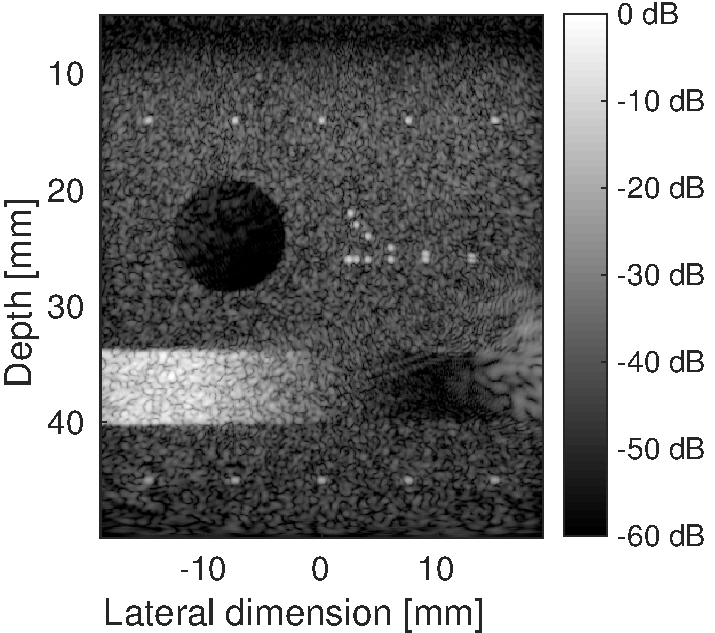
\includegraphics[width=\CohSubFigWidth]{Figures/das_dataset_rf_numerical_transmission_1_nbPW_1.pdf}}
\begin{figure*}[htb]
	% Maximum length
	\hfill%
	\subcaptionbox{\label{fig_numerical_DAS}}{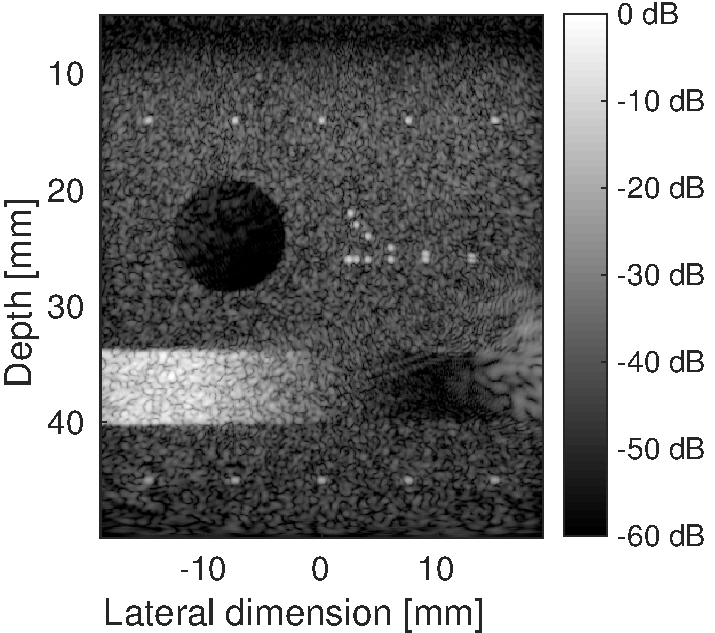
\includegraphics[height=\CohSubFigHeight]{Figures/das_dataset_rf_numerical_transmission_1_nbPW_1.pdf}}\hfill%
	\subcaptionbox{\label{fig_numerical_DAS_5}}{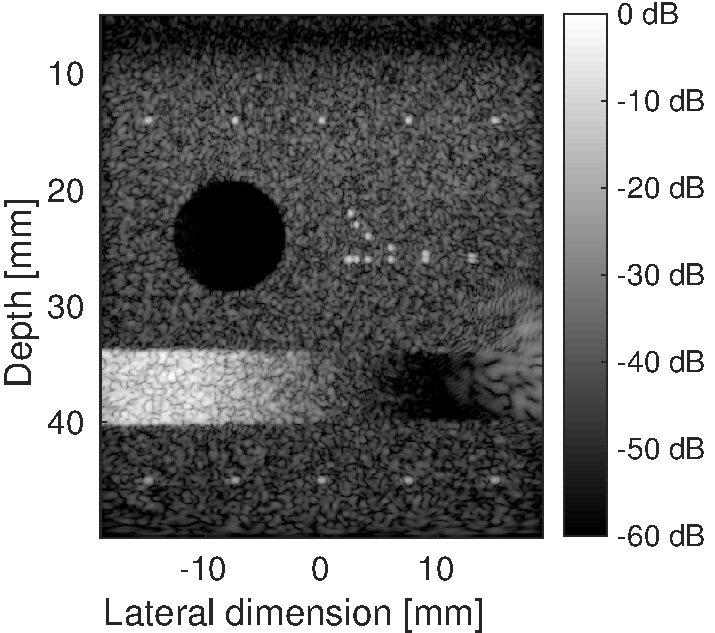
\includegraphics[height=\CohSubFigHeight]{Figures/das_dataset_rf_numerical_transmission_1_nbPW_5.pdf}}\hfill%
	\subcaptionbox{\label{fig_numerical_FISTA}}{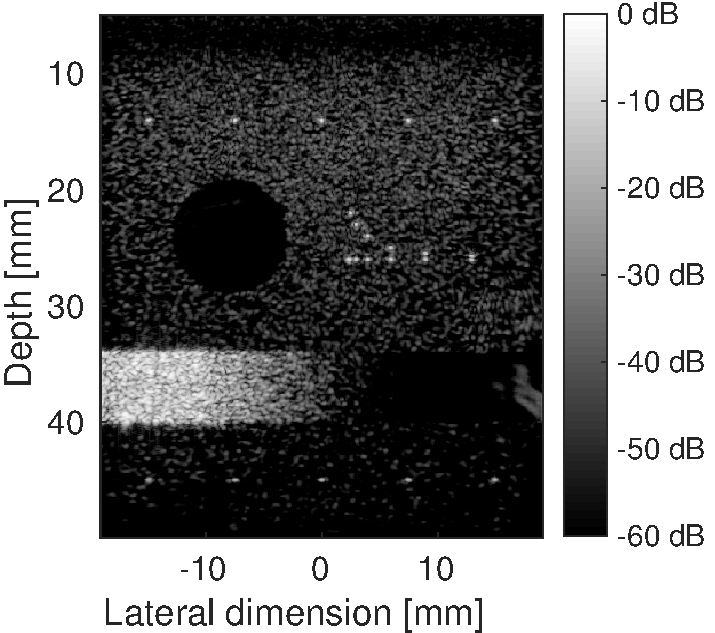
\includegraphics[height=\CohSubFigHeight]{Figures/FISTA_dataset_rf_numerical_transmission_1_nbPW_1.pdf}}\hfill%
	\subcaptionbox{\label{fig_numerical_FISTALP}}{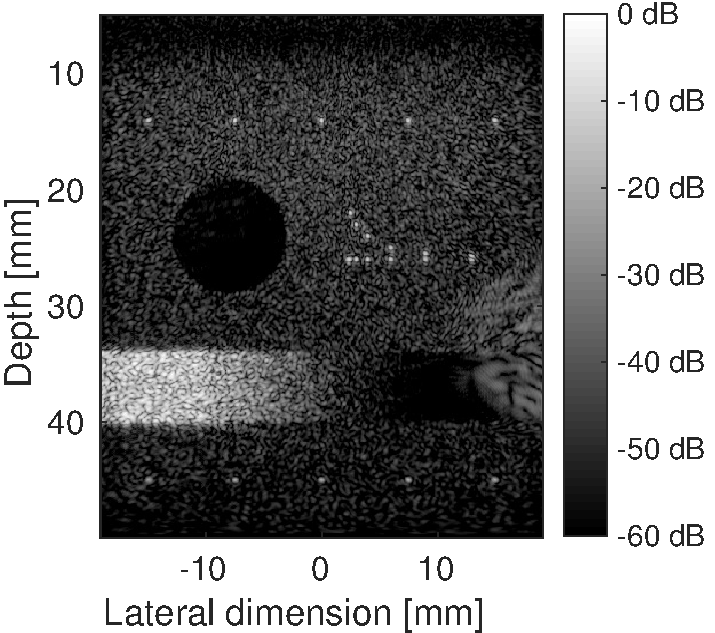
\includegraphics[height=\CohSubFigHeight]{Figures/FISTALP_dataset_rf_numerical_transmission_1_nbPW_1.pdf}}\hfill\null%
	
	\hfill%
	\subcaptionbox{\label{fig_carotid_DAS}}{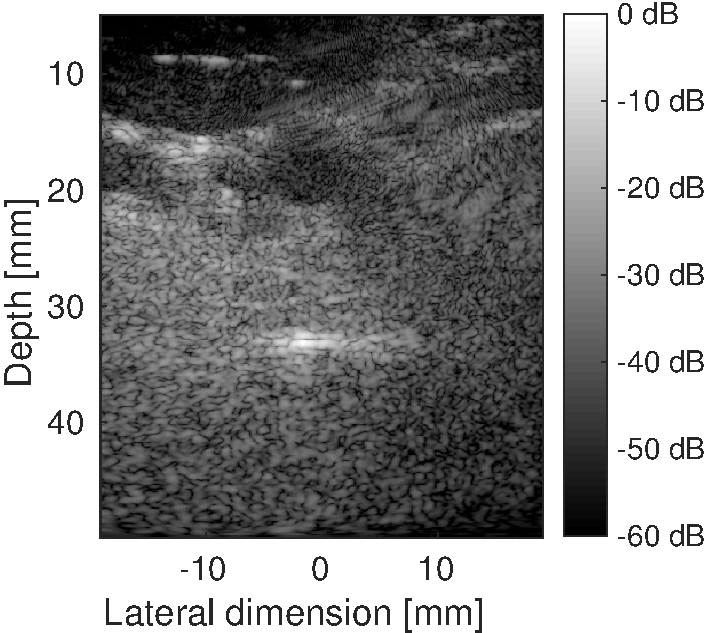
\includegraphics[height=\CohSubFigHeight]{Figures/das_carotid_cross_expe_dataset_rf.pdf}}\hfill%
	\subcaptionbox{\label{fig_carotid_DAS_5}}{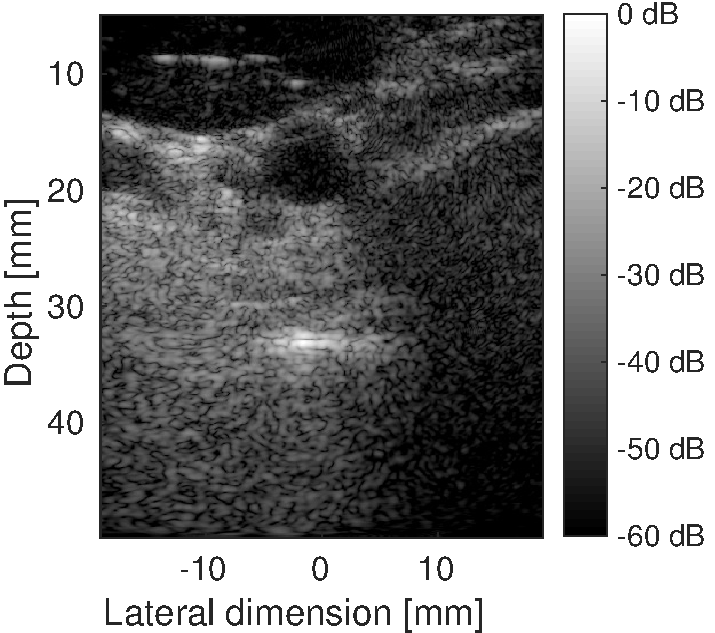
\includegraphics[height=\CohSubFigHeight]{Figures/das_carotid_cross_expe_dataset_rf_5PWs.pdf}}\hfill%
	\subcaptionbox{\label{fig_carotid_FISTA}}{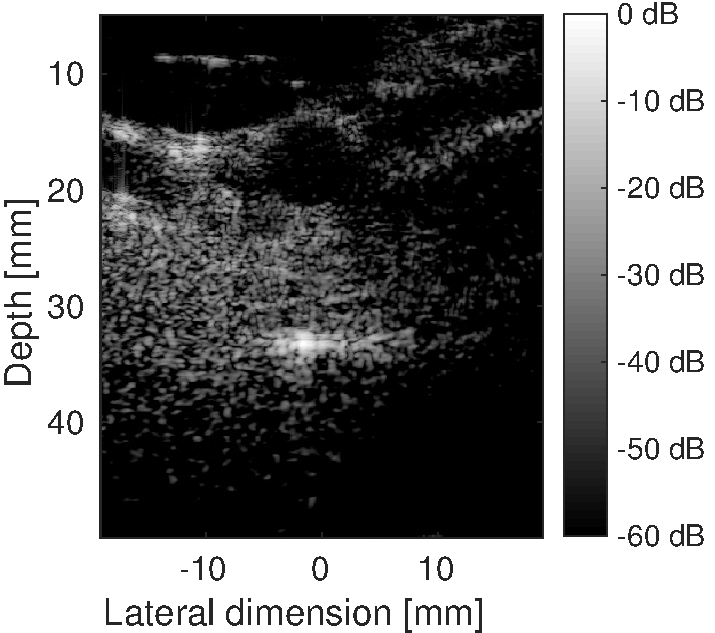
\includegraphics[height=\CohSubFigHeight]{Figures/FISTA_carotid_cross_expe_dataset_rf.pdf}}\hfill%
	\subcaptionbox{\label{fig_carotid_FISTALP}}{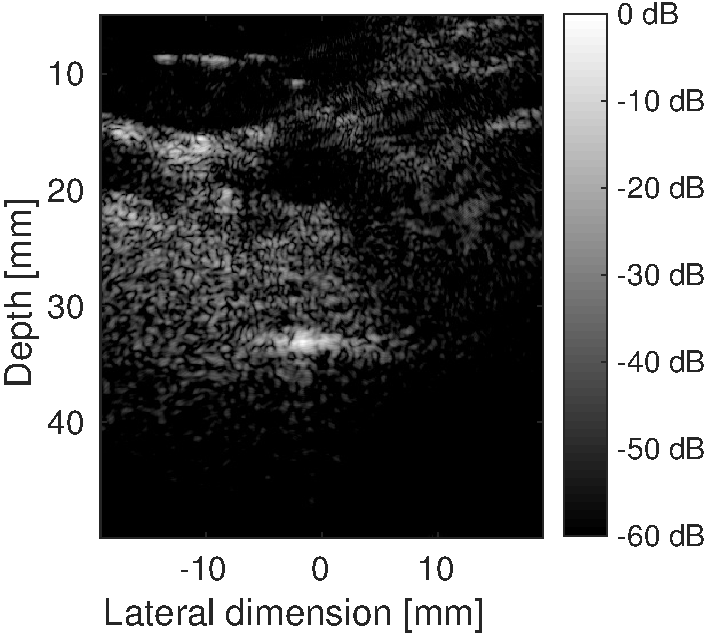
\includegraphics[height=\CohSubFigHeight]{Figures/FISTALP_carotid_cross_expe_dataset_rf.pdf}}\hfill\null%
	\caption{Image of the numerical phantom reconstructed with (a) DAS - 1 PW insonification, (b) DAS - 5 PW insonifications, (c) USSR-SA - 1 PW insonification, (c) USSR - $\ell_p$ - 1 PW insonification; Image of the \textit{in-vivo} carotid reconstructed with (e) DAS - 1 PW insonification, (f) DAS - 5 PW insonifications, (g) USSR-SA - 1 PW insonification, (h) USSR-$\ell_p$ - 1 PW insonification.}
	\label{fig_Bmode}
\end{figure*} 

The CNR, axial and lateral resolution computed on the numerical phantom, summarized in Table~\ref{tab_results_numerical}, show that both reconstruction methods recover high resolution images. Regarding the contrast, the method coupled with SA has a higher CNR than DAS with \num{1} PW insonification but significantly lower than DAS with 5 PW insonifications, due to the decrease of speckle density induced by the higher resolution.

Visual assessment of the recovered B-mode images, displayed on Figure~\ref{fig_Bmode} confirms the results obtained with the metrics. Regarding the \textit{in-vivo} carotids, the proposed methods lead to significantly higher quality images than the ones obtained with the DAS algorithm.

Regarding the timings, \num{200} iterations of FISTA take around \SI{4.5}{\second} with the current implementation~(not optimized) on an NVIDIA GeForce GTX 1080 Ti GPU, for both the $\ell_p$-norm and the SA model. This can be explained by the fact that most of the time is spent computing the measurement model and the adjoint operator. We believe that a substantial gain may be achieved by optimizing the code.   
\section{Conclusion}
\label{sec_conclusion}
We propose USSR, an UltraSound Sparse Regularization framework based on sparse regularization, as an alternative to DAS imaging. We describe matrix-free formulations of the measurement model and its adjoint in the context of PW imaging, which allow us to provide fast reconstructions with a low memory footprint. The framework is equipped with two models for the priors, namely $\ell_p$-norm prior in the image domain and $\ell_1$-norm prior prior in a sparsity averaging model. The evaluation is performed on the publicly available PICMUS dataset, so that the results presented in this work are reproducible, and show that the proposed method yields improved image quality compared to state-of-the art methods. 

\section*{Acknowledgements}
This work was supported in part by the UltrasoundToGo RTD project (no. 20NA21\_145911), evaluated by the Swiss NSF and funded by Nano-Tera.ch with Swiss Confederation financing.
 
\bibliographystyle{IEEEtran}
% argument is your BibTeX string definitions and bibliography database(s)
\bibliography{IEEEabrv,ius2017}

\end{document}
